% ============================================================== 3. Materials and methods
\section{Materials and methods}
\label{sec:methods}

\subsection{Study overview and research questions}
\label{sec:overview}

Fig.~\ref{fig:framework} summarizes the study. We trained federated, personalized, centralized and
local models on the six clients of Fed-ISIC2019, once on image-level splits (the common practice) and
once on lesion-grouped splits, and evaluated accuracy, calibration and conformal coverage overall and per
client. Four research questions organize the methods, results and discussion:

\begin{description}
\item[RQ1] With a lesion-grouped split, how reliable are federated accuracy, calibration and conformal
  coverage overall, per client, on clients unseen in training, and under a shift to smartphone images?
\item[RQ2] How unevenly is lesion leakage distributed across the Fed-ISIC2019 clients, and how much does
  it change apparent accuracy, method rankings, calibration and conformal coverage?
\item[RQ3] Does personalization improve per-client results under a lesion-grouped split, and do local
  and personalized models show the largest apparent gain from leakage (hypothesis H3b)?
\item[RQ4] Can a client-specific conformal threshold that borrows strength from the other clients
  reduce low-coverage calibration draws in small clients without enlarging prediction sets?
\end{description}

The experiments were: E0, reproduction of the published benchmark on the official split; E1,
image-level versus lesion-grouped splits for three encoder configurations; E2, eight training methods on
both split types; E3, calibration; E5, federated conformal prediction on in-federation models; E6,
leave-one-client-out (LOCO) models and a smartphone-image stress test; E7, personalized models and the
final test of H3b; E8, a randomized sibling-exposure experiment on fixed test images; and E9,
capacity-matched classifier heads for model~B. The optional experiment E4 was not run. Seeds differed
between experiments (Supplementary~S10 gives the full run matrix): three for E0, E1, E6 and E8, five for E2, E7
and E9. Confirmatory tests followed the protocol version that was fixed before the corresponding runs
(Section~\ref{sec:prereg}); all other analyses are labelled secondary, post hoc or exploratory.

\begin{figure*}[!t]
  \centering
  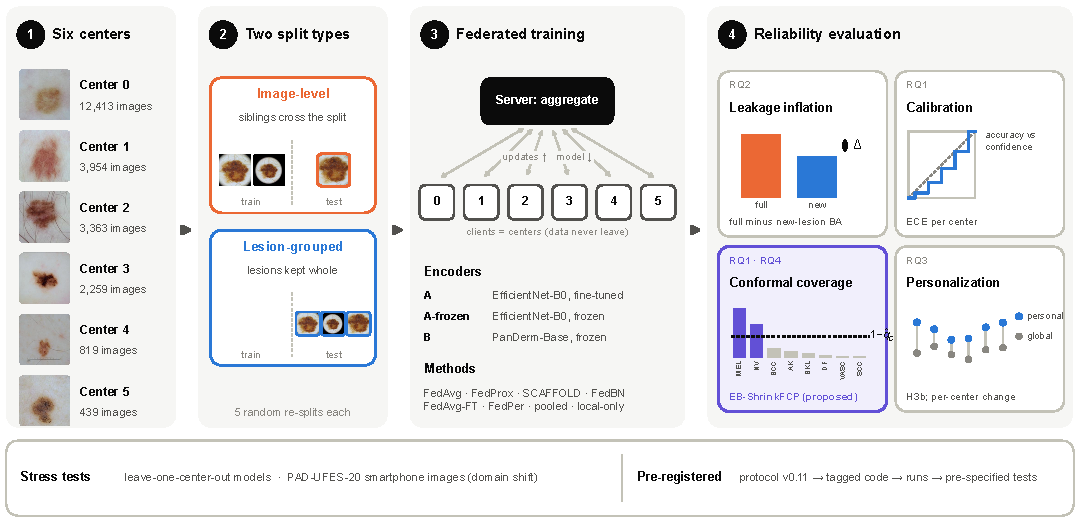
\includegraphics[width=\textwidth]{Fig2_framework}
  \caption{Study framework. (1) Six Fed-ISIC2019 clients (acquisition sources) with one example image
  each. (2) Models are trained and evaluated on image-level splits, in which images of one lesion can
  fall on both sides, and on lesion-grouped splits, in which they cannot (three to five random re-splits
  of each type, depending on the experiment; Supplementary~S10). (3) Simulated federated training with three
  encoder configurations and up to eight methods: images stay with their client during federated
  training, while the centralized baseline pools them. (4) Four evaluation questions; the proposed
  EB-ShrinkFCP is highlighted. Bottom: stress tests and the version-controlled protocol. Images: ISIC
  2019 (CC-BY-NC 4.0).}
  \label{fig:framework}
\end{figure*}

\subsection{Datasets}
\label{sec:data}

\paragraph{Fed-ISIC2019} We used the Fed-ISIC2019 benchmark of FLamby \cite{flamby2022} (commit
\texttt{edacf54}): 23,247 dermoscopy images from the ISIC 2019 challenge
\cite{codella2018isic,tschandl2018ham,combalia2019bcn}, labelled with eight diagnostic classes
(melanoma, MEL; melanocytic nevus, NV; basal cell carcinoma, BCC; actinic keratosis, AK; benign
keratosis, BKL; dermatofibroma, DF; vascular lesion, VASC; squamous cell carcinoma, SCC). FLamby defines
six clients by acquisition source (Table~\ref{tab:dataset}): BCN20000 (client~0), MSK (client~4) and four
HAM10000 subsets, three of which (clients 1, 2 and 5) come from one institution in Vienna with different
acquisition devices. FLamby calls the clients ``centers''; we call them clients because they are acquisition sources rather
than six independent hospitals. Images were preprocessed with FLamby's procedure (shorter
edge resized to 224 pixels, color constancy with power 6).

Lesion identifiers were taken from the HAM10000 metadata (clients 1, 2, 3 and 5) and the ISIC 2019
metadata (clients 0 and 4). All 23,247 images have an identifier; none equals its image name, no lesion
carries two diagnoses, and the data contain 11,847 lesions. Nine lesions have images in two clients
(clients 1 and 2, both from the Vienna institution), which is why the per-client lesion counts in
Table~\ref{tab:dataset} sum to 11,856. The number of images per lesion ranges from one to 31 (median 1;
3.47 on average in client~0). Patient identifiers are not available for Fed-ISIC2019, so our splits are
lesion-disjoint but not necessarily patient-disjoint. Supplementary~S1 gives the per-client and per-class
counts and the identifier checks.

\inputtable{Table1_dataset}

\paragraph{PAD-UFES-20} As a domain-shift stress test we used PAD-UFES-20 \cite{pacheco2020pad}:
2,298 clinical photographs taken with smartphones (not dermoscopy) from 1,373 patients. Its six
diagnoses were mapped to the Fed-ISIC2019 classes (MEL$\to$MEL, NEV$\to$NV, BCC$\to$BCC,
ACK$\to$AK, SEK$\to$BKL, SCC$\to$SCC). This is a closed-set transfer: model probabilities were
restricted to the six shared classes and renormalized before any metric or conformal threshold was
computed, on the source and the target data alike. Lesion numbers in the PAD-UFES-20 metadata are
reused across patients (250 numbers occur under two patient identifiers, mostly with different
diagnoses; the pair of patient and lesion number identifies 1,891 lesions), so all PAD-UFES-20 analyses
were grouped by patient. No model was trained or fine-tuned on PAD-UFES-20.

\subsection{Data splits}
\label{sec:splits}

Three kinds of split were used (files, checksums and realized sizes are in the code repository and
Supplementary~S1).
\emph{Official}: FLamby's fixed image-level split, used to reproduce published results (E0) and to
report the leakage of the benchmark as distributed.
\emph{Image-level} re-splits: 20\% of each client's images form the test set, stratified by class,
irrespective of lesion.
\emph{Lesion-grouped} re-splits: 20\% of each client's lesions, with all their images, form the test set,
under class quotas; the nine lesions with images in two clients were always kept in training. Because the
two split types draw 20\% of images and 20\% of lesions respectively, their training sets differ by less
than 1\% in images (about 16,700--16,800) but not in lesions (about 9,350 versus 8,500), and their test
sets differ in composition (Supplementary~S1). From E1 onwards, 10\% of each client's training lesions
were moved to a validation fold, grouped by lesion in both split types; the validation fold was used only
for temperature scaling. In the lesion-grouped splits no lesion occurs in more than one of training,
validation and test. In the image-level splits this holds for training and validation, but 6.5\% of the
test images belong to a lesion that is in the validation fold and not in training; these images were
counted as new (they were not used for training) and are examined in a sensitivity analysis. The split
seed and the training seed of a run share the same number, so split and initialization randomness are not
varied independently.

For a model trained on an image-level split, a test image is \emph{leaked} if its lesion has images in
the training set of any client and \emph{new} otherwise. The \emph{leakage rate} of a client is the
share of its image-level test images that are leaked (Table~\ref{tab:dataset}; Fig.~\ref{fig:leakage}b).
Leakage through another client was rare (0.1\% of test images, mainly in client~1, whose lesions have
one image each but nine of which also occur in client~2).

\subsection{Models}
\label{sec:models}

We used three encoder configurations. \emph{Model A} is EfficientNet-B0 \cite{tan2019efficientnet}
pretrained on ImageNet \cite{deng2009imagenet} and fully fine-tuned, the FLamby baseline. \emph{Model
A-frozen} uses the same network and weights, frozen, with a federated linear head. It is a control for
full fine-tuning that keeps architecture and initial weights fixed; it also differs from model~A in the
optimizer schedule, the number of updates and the use of cached augmented views, so it does not isolate
fine-tuning completely. \emph{Model B} is PanDerm-Base \cite{yan2025panderm}, a ViT-B/16
\cite{dosovitskiy2021vit} dermatology foundation model (checkpoint
\texttt{panderm\_bb\_data6\_checkpoint-499.pth}, SHA-256 \texttt{be1e0fb1\ldots0ac1ff1}, full hash in the
repository), frozen, with a federated head on the 768-dimensional
CLS token after the final layer normalization. ISIC 2019, HAM10000, BCN20000 and PAD-UFES-20 are not
listed among PanDerm's pretraining sources, but overlap could not be ruled out, so results for model~B
are reported with this caveat.

For the frozen encoders, embeddings were computed once, with the encoder in evaluation mode, for one
plain view (FLamby's test transform: center crop of 200 pixels and ImageNet normalization; resized
bilinearly to 224 pixels for PanDerm) and for five augmented views (FLamby's training transforms, with
the random seed of view $v$ of image $i$ fixed to $1{,}000{,}003\,v+i$) of every image. Training draws one
of the five views at random each time an image is used; validation and test use the plain view.
Embeddings were centered with the mean over all training images and views, computed federatedly from
per-client sums; the mean excludes validation and test images and, for LOCO models, the held-out
client. The number of local updates per round for the federated heads ($U=6{,}400$ minibatch steps of 64
images) was fixed once per encoder by a pre-specified rule on the lesion-grouped split of seed~0
(doubling $U$ from 100 while the pooled training loss fell by more than 1\% in the last of nine rounds)
and then used unchanged for every split, seed and method. Because clients differ in size, $U$ corresponds
to about 46 passes over the training data of client~0 per round and about 1,300 passes for client~5.

\subsection{Federated and baseline methods}
\label{sec:methods-fl}

We compared up to eight training methods. \emph{FedAvg} \cite{mcmahan2017fedavg}, \emph{FedProx}
\cite{li2020fedprox} ($\mu=0.001$) and \emph{SCAFFOLD} \cite{karimireddy2020scaffold} (server learning
rate 1.0) learn one global model. Three personalized methods adapt it to each client:
\emph{FedBN} \cite{li2021fedbn} keeps the batch-normalization weights and biases local (model~A only, as
linear heads have none); \emph{FedAvg-FT} fine-tunes the final FedAvg model for three local SGD steps per
client, a pre-specified light personalization that was not tuned; and \emph{FedPer}
\cite{arivazhagan2019fedper} keeps the classifier local and averages the remaining parameters (for
model~A the final linear layer is local). For models with a frozen encoder, a client-specific linear head
would be identical to local training, so FedPer used a two-layer head (768--256--8, ReLU) with a
federated hidden layer and a client-specific output layer. Because this head has more capacity than the
linear heads of the other model~B methods, E9 trained FedAvg, pooled and local-only models with the same
two-layer head. \emph{Pooled} training is the centralized reference, and \emph{local-only} trains one model
per client on its own data.

Federated training followed FLamby: 9 rounds of 100 local updates (model~A; 6,400 images per client and
round) or $U$ updates (frozen encoders), SGD with learning rate 0.01 and batch size 64, weighted focal loss
\cite{lin2017focal} ($\gamma=2$) with FLamby's fixed class weights (taken unchanged from FLamby's code
for all splits), and aggregation of all trainable parameters weighted by the number of training images.
Batch-normalization running statistics are buffers, not parameters, and stay with each client in all
methods; FedBN additionally keeps the batch-normalization weights and biases local. The global FedAvg,
FedProx and SCAFFOLD model was evaluated as the copy held by the first participating client, including
that client's running statistics (FLamby's convention); for a LOCO model this is a client other than the
held-out one, and no statistics were adapted to the held-out client. Pooled and local-only models used
Adam \cite{kingma2015adam} (learning rate $5\times10^{-4}$, batch 64, 20 epochs). These optimizer and
budget differences follow the benchmark and make pooled and local-only models operational references
rather than matched controls. Model~A started from ImageNet weights with a newly initialized output layer;
all heads on frozen encoders used PyTorch's default initialization. No hyper-parameter was tuned on a test
set. Model~A FedAvg was also trained for 27 rounds, because an under-trained model may fit its training
lesions less and understate leakage. For RQ1, LOCO FedAvg models were trained on five clients and
evaluated on all six (six held-out clients, seeds 0--2, models A and B). Personalized models were
evaluated on each client with that client's own model.

\paragraph{Randomized sibling exposure (E8)} The leakage contrast defined below compares different test
images and is therefore observational. To estimate the effect of having a sibling image in training on
the \emph{same} test images, E8 used the lesion-grouped splits of seeds 0--2. Each test lesion with at
least two test images (about 1,000 lesions per seed) contributed one randomly drawn \emph{target} image;
its other images were its \emph{siblings}. Target lesions were randomized into two groups, stratified by
client and class and paired by number of siblings. In arm~1 the siblings of group~1 were added to the
training set of their client and those of group~2 were removed; arm~2 did the reverse. All other images
were identical in both arms, and the training sets differed by less than 0.2\% in size. Every target image
is therefore predicted once with and once without its siblings in training, by models with the same
recipe and seed. E8 trained FedAvg, FedPer, pooled and local-only models for models A and B, and FedAvg,
pooled and local-only models for A-frozen. The design and its primary test were added to the protocol
(version 0.12) after all other results were known and before any E8 model was trained.

\subsection{Evaluation metrics}
\label{sec:metrics}

\paragraph{Accuracy} Balanced accuracy (BA), the mean of per-class recalls over the classes present, was
computed on the pooled test set (FLamby's benchmark metric) and as the mean of the six per-client values.
Per-client BA averages over the classes present in that client's test set, which differ between clients
(Supplementary~S1).

\paragraph{Apparent leakage inflation} For a model trained on an image-level split, the \emph{apparent
inflation} is
\begin{equation}
  \Delta_{\text{app}} = \mathrm{BA}_{\text{full}} - \widetilde{\mathrm{BA}}_{\text{new}},
  \label{eq:inflation}
\end{equation}
the BA on the full image-level test set minus a standardized BA on its new-lesion subset, for the same
model. Let $r_{c,k}$ be the recall of class $k$ among the new-lesion test images of client $c$ and $N_{c,k}$
the number of all test images of class $k$ in client $c$. Then $\widetilde{\mathrm{BA}}_{\text{new}}$ is
the mean over classes $k$ of $\sum_c N_{c,k} r_{c,k}/\sum_c N_{c,k}$, where the sums run over the clients
with at least one new-lesion image of class $k$; classes with fewer than five new-lesion images in total
are dropped from both terms. $\Delta_{\text{app}}$ is an observational contrast between two groups of test
images. Within a class it equals the leaked share times the difference in recall between leaked and new
images, so it can also reflect differences in difficulty or multiplicity between leaked and new lesions,
and it grows mechanically with the leakage rate. We therefore report two further estimands: the
\emph{retrained-split difference}, the BA of the image-level model on its own test set minus the BA of the
lesion-grouped model on its own test set (different models and test sets), and the \emph{exposure effect}
of E8, the BA of the target images when their siblings were in training minus their BA when they were
not (same images; classes with at least five target images). For H3b, inflation was computed within each
client without standardization.

\paragraph{Rankings} Methods were ranked by mean BA over five seeds on each split type, and agreement
between the image-level and lesion-grouped rankings was measured with Kendall's $\tau_b$ (no ties occurred). To separate leakage from training noise, we compared the
agreement of single-seed rankings across split types (mean over 25 seed pairs) with a noise floor, the
mean agreement of single-seed rankings from different seeds within one split type (10 pairs per split
type); the pairs share seeds and are not independent. Seed-level BA and paired differences to FedAvg are given in
Supplementary~S10.

\paragraph{H3b} The mean inflation of the local and personalized group (local-only, FedAvg-FT, FedBN
and FedPer for model~A; local-only, FedAvg-FT and FedPer for model~B) minus that of FedAvg, averaged over
clients 0, 2 and 3 with weights proportional to their new-lesion counts. These clients were fixed in
protocol version 0.8, before any model was trained, as the clients with substantial leakage and enough
new-lesion test images in the official split (182, 185 and 229). A secondary dose--response analysis related each
method's per-client inflation to the client's leakage rate by weighted least squares over the six clients;
with six clients, one of them (client~0) with most of the leakage, this slope is descriptive.

\paragraph{Calibration} We report the top-label expected calibration error (ECE) with 15 equal-width
bins \cite{naeini2015ece,guo2017calibration}, class-wise ECE \cite{kull2019beyond}, the negative
log-likelihood (NLL) and the Brier score \cite{brier1950}, overall and per client. Probabilities were
temperature-scaled \cite{guo2017calibration}: each client fitted a temperature on its validation lesions
by minimizing the NLL, and the global temperature was their mean weighted by validation images, a
heuristic that needs no exchange of logits; the NLL-optimal temperature on the pooled validation set is
reported as a sensitivity analysis. All methods, including personalized ones, used the global temperature
of their own predictions. Because binned ECE is biased upwards in small samples, contrasts between the
new-lesion subset and the full test set were also computed against random subsets of the full test set
with the same size and the same client-by-class counts (200 draws), and for NLL and Brier score against
the full test set reweighted to the client-by-class composition of the new-lesion subset. For model~A
FedAvg we also evaluated Monte Carlo dropout \cite{gal2016dropout} (20 passes through the network's single
dropout layer before the classifier, $p=0.2$).

\subsection{Federated conformal prediction}
\label{sec:conformal}

\paragraph{Scores and sets} With temperature-scaled softmax probabilities $\hat p(y\mid x)$ (global
temperature), we used the LAC score $s(x,y)=1-\hat p(y\mid x)$ \cite{sadinle2019lac} (primary) and the
non-randomized APS score \cite{romano2020aps}, $s(x,y)=\sum_{y'}\hat p(y'\mid x)\,\mathbb{1}[\hat
p(y'\mid x)\ge \hat p(y\mid x)]$ (ties included). For a threshold $q$, the prediction set is
\begin{equation}
  C(x)=\{\,y: s(x,y)\le q\,\},
  \label{eq:set}
\end{equation}
which may be empty. The target coverage was $1-\alpha=0.9$ (also 0.8 and 0.95)
\cite{angelopoulos2023gentle}.

\paragraph{Calibration and evaluation data} Each client's lesion-grouped test set served as a held-out
pool for conformal analysis. In each of 100 draws, its lesions were split at random into a calibration
half and an evaluation half; thresholds were computed from the calibration half only and coverage and set
size were measured on the evaluation half. These pools were used to evaluate several methods, so they are
held out from training but not an untouched final test set. Split conformal prediction guarantees
marginal coverage when calibration and test units are exchangeable
\cite{vovk2005algorithmic,angelopoulos2023gentle}. Here the units are images, and images of one lesion are
correlated; random assignment of whole lesions makes the lesions, but not the individual images,
exchangeable \cite{lee2023hierarchical,dunn2022hierarchical}. We therefore treat image-level coverage as an
empirical quantity, and as a sensitivity analysis we kept one random image per lesion in both halves, so
that calibration and evaluation units are independent lesions and the target is a random image of a new
lesion.

\paragraph{Thresholds} Let client $c$ have $m_c$ calibration images in $n_c$ lesions, and let $q_c$ be
its own conformal quantile, the $\lceil (m_c+1)(1-\alpha)\rceil$-th smallest calibration score (1 if this
rank exceeds $m_c$). We compared seven rules:
\emph{global}, one threshold from the pooled scores of all clients, computed from 1,000-bin score
histograms that each client shares and rounded up to the upper bin edge;
\emph{client-wise}, $q_c$ for each client;
\emph{sample-weighted}, $\sum_c (m_c/m)\,q_c$ for every client;
\emph{FCP} \cite{lu2023fcp}, the pooled threshold at level $\lceil (m+K)(1-\alpha)\rceil/m$ for $K$
clients, the rank correction of Lu et al.\ for a guarantee on the mixture of clients under partial
exchangeability, here computed from the same histograms;
\emph{ShrinkFCP} (pre-specified for RQ4), $w_c q_c + (1-w_c) q_g$ with $w_c=n_c/(n_c+k)$, the global
threshold $q_g$ and $k$ the median of $n_c$ over clients;
\emph{EB-ShrinkFCP}, introduced next; and, as a post hoc comparator, a \emph{label-shift-weighted}
threshold (LSW) for each client, the weighted quantile of the pooled calibration scores with weights
$\hat\pi_c(y)/\hat\pi(y)$ from calibration class frequencies and a conservative weight for the test point
\cite{podkopaev2021labelshift,plassier2023labelshift}, computed from per-class score histograms. Global,
sample-weighted and FCP thresholds target coverage on the mixture of clients, not per client
\cite{lu2023fcp}; client-wise thresholds target each client. Personalized FCP with localization
\cite{min2025pfcp}, listed in the protocol as a comparator, was not implemented because its threshold
rule could not be verified from the available description and no code was found.

\paragraph{EB-ShrinkFCP} ShrinkFCP assumes that small clients differ from the global threshold only by
sampling noise. When a client's score distribution is genuinely shifted, shrinking toward a shared
threshold imports that shift. EB-ShrinkFCP therefore estimates how much the clients differ beyond sampling
noise and shrinks only by that much, using the normal-means empirical-Bayes idea
\cite{efron1975stein} with the random-effects estimator of DerSimonian and Laird
\cite{dersimonian1986meta} (Algorithm~\ref{alg:eb}). Each client shares only its quantile and an estimate
of its sampling variance. The variance is obtained from the spread of order statistics around the
quantile, a standard approximation to the standard error of a sample quantile, with the spacing widened
by the average number of images per calibration lesion, $m_c/n_c$, as a heuristic allowance for
correlated images; this factor is not a general design effect for unequal clusters, and its adequacy was
checked post hoc with the lesion bootstrap and in a simulation (Supplementary~S6, S15 and S16). The server combines the quantiles into a
between-client variance $\tau^2$ and a precision-weighted mean $\bar q$, and returns
\begin{equation}
  \hat q_c = w_c\,q_c + (1-w_c)\,\bar q, \qquad w_c=\frac{\tau^2}{\tau^2+\sigma_c^2}.
  \label{eq:eb}
\end{equation}
When the clients disagree far beyond their sampling noise, $w_c\to1$ and each client keeps its own
threshold; when they agree, noisy (small) clients borrow from the others. The mean $\bar q$ uses the
within-client precisions $1/\sigma_c^2$, as in the pre-specified rule; a random-effects mean with weights
$1/(\sigma_c^2+\tau^2)$ would be an alternative. The rule has no validation-tuned shrinkage parameter; its
fixed choices are the variance floor of $10^{-6}$ and the order-statistic spacing. Unshrunk client-wise
thresholds inherit the split-conformal guarantee under within-client exchangeability; shrinkage toward
$\bar q$ removes that guarantee, so EB-ShrinkFCP is an empirical rule whose per-client coverage was
assessed empirically.

\begin{algorithm}[!t]
\caption{EB-ShrinkFCP: per-client conformal thresholds with empirical-Bayes shrinkage.}
\label{alg:eb}
\begin{algorithmic}[1]
\Require miscoverage $\alpha$; at each client $c=1,\dots,K$: calibration scores $s_{c,(1)}\le\dots\le s_{c,(m_c)}$ from $n_c$ lesions
\For{each client $c$ \textbf{(locally)}}
  \State $p_c \gets \lceil (m_c+1)(1-\alpha)\rceil/m_c$, \quad $r \gets \lceil p_c m_c\rceil$
  \State $q_c \gets s_{c,(r)}$ \quad (1 if $r>m_c$)
  \State $d \gets \big\lceil \sqrt{m_c\,\min(p_c,1)\,(1-\min(p_c,1))\cdot m_c/n_c}\,\big\rceil$
  \State $\sigma_c \gets \tfrac12\big(s_{c,(r+d)}-s_{c,(r-d)}\big)$ \quad (ranks clipped to $[1,m_c]$; rank $>m_c$ counts as 1)
  \State send $(q_c,\sigma_c^2)$ to the server
\EndFor
\State \textbf{Server:} $v_c \gets 1/\max(\sigma_c^2,10^{-6})$, \quad $\bar q \gets \sum_c v_c q_c / \sum_c v_c$
\State $Q \gets \sum_c v_c (q_c-\bar q)^2$, \quad $\tau^2 \gets \max\!\Big(0,\ \dfrac{Q-(K-1)}{\sum_c v_c-\sum_c v_c^2/\sum_c v_c}\Big)$
\For{each client $c$}
  \State $w_c \gets \tau^2/(\tau^2+\sigma_c^2)$ \quad ($w_c=0$ if $\tau^2=0$)
  \State $\hat q_c \gets w_c q_c + (1-w_c)\,\bar q$ \Comment{returned to client $c$}
\EndFor
\end{algorithmic}
\end{algorithm}

\paragraph{RQ4 metric} Client-wise calibration gives each client about 90\% coverage on average, so the
remaining risk in small clients lies in unlucky calibration draws. For each model and client we took the
10th percentile of evaluation coverage over the 100 draws (lower-tail coverage, q10), then the minimum over
clients, and averaged this \emph{worst-client q10} over models. Because each draw changes both halves,
q10 combines threshold variability with the sampling noise of the evaluation half: in client~5 one
evaluation image is about 2.3 coverage points. Gains between methods are paired on the same draws. As
sensitivity analyses we estimated q10 from 1,000 draws and from five independent sets of 100 draws, and we
isolated threshold variability by fixing the evaluation half and redrawing only the calibration lesions
(lesion bootstrap of the other half, 100 draws, five fixed evaluation halves per model).

\paragraph{LOCO conformal evaluation} For test~5b, each of the 18 LOCO models per encoder produced scores on
the lesion-grouped test sets of all six clients, including the client held out of its training; for every
model, thresholds were then calibrated and evaluated as above. The held-out client is therefore unseen in
training but calibrated with its own labelled lesions; this is not target-label-free external validation.

\paragraph{Smartphone stress test} On PAD-UFES-20, conformal thresholds were either (i) transferred,
computed from all Fed-ISIC2019 lesion-grouped test scores after the six-class restriction and the same
global temperature as on the target, or (ii) recalibrated on a random half of the PAD-UFES-20 patients and
evaluated on the other half, 100 times. These are two deployment scenarios, without and with labelled
target data.

\subsection{Protocol, pre-specified tests and statistical analysis}
\label{sec:prereg}

The protocol specified research questions, splits, models, metrics and success criteria before the
corresponding experiments \cite{nosek2018preregistration}. It was not deposited in an external registry;
instead, each version and each pre-run state of the code was committed and tagged in a git repository that
was pushed to GitHub before the runs it governs, and the full history is released. Supplementary~S9 lists every
version with its date, the results available when it was written and what it changed. Versions 0.1--0.10
(26--30 October 2026) were written, and revised after five methodological reviews, before any experiment
was run. Version 0.11 (3 November) was written after E0--E5 and before any LOCO model was trained, and
version 0.12 (7 November) after all other results and an external review of the manuscript, and before
any E8 or E9 model was trained. The pre-specified tests were:
\begin{itemize}
  \item \emph{Gate 1} (pipeline check): model~A FedAvg pooled BA on the official split within
    $0.657\pm0.05$, the FedAvg baseline reported in the FENDA-FL study of Tavakoli et al.\
    \cite{tavakoli2024fendafl} (margin fixed in version 0.4; meeting it is a replication tolerance, not
    a test of equivalence);
  \item \emph{Gate 2} (primary RQ2 outcome, v0.4): model~A FedAvg apparent inflation
    (Eq.~\ref{eq:inflation}) of at least 2 points with the 95\% interval above zero;
  \item \emph{H3b} (RQ3, v0.8): the H3b contrast with the 95\% interval above zero;
  \item \emph{RQ4} (v0.8--0.10): for each of models A and B, ShrinkFCP raises the worst-client q10 by at
    least 2 points over the better of global and client-wise calibration, with the interval of the gain
    above zero, a mean set size at most 10\% larger than the reference's, and every client's mean coverage
    at least 0.89 (LAC, $\alpha=0.1$, lesion-grouped FedAvg models);
  \item \emph{5b} (v0.11): the same criterion for EB-ShrinkFCP on the LOCO models (18 per encoder);
  \item \emph{PAD-UFES-20 transfer} (implementation notes fixed on 6 November 2026, before any
    PAD-UFES-20 prediction): transferred thresholds are reported as failing if coverage is below
    $1-\alpha$ with the patient-bootstrap interval excluding $1-\alpha$;
  \item \emph{E8} (v0.12): model~A FedAvg exposure effect of at least 2 BA points with the 95\% interval
    above zero.
\end{itemize}
RQ4 and 5b require success for each encoder separately; ``at least 2 points with the interval above
zero'' requires a point estimate of 2 points or more and a lower interval bound above zero, not an
interval above 2 points. Gate~2 is the single primary outcome; all other tests are secondary, and no
correction for multiplicity was applied, so their intervals are not independent confirmations.
Analyses not in the protocol are labelled post hoc or exploratory; the sensitivity analyses added after
the external review are listed in Supplementary~S9.

Unless stated otherwise, intervals are 95\% percentile intervals from a lesion-level cluster bootstrap
\cite{field2007cluster} of the test sets (2,000 replicates; 1,000 for calibration
contrasts), with the trained models fixed and seeds averaged inside each replicate; they reflect
test-sample uncertainty, not retraining variability, which is shown by the seed-level results in
Supplementary~S10. For the conformal gains, each replicate resampled the test lesions and redrew 20
calibration draws shared by all methods, so that gains are paired. In the pre-specified analysis, copies of
a resampled lesion were treated as distinct lesions and could therefore fall into both halves; a corrected
bootstrap that keeps the copies of a lesion together, with 20 and with 100 draws per replicate, is
reported in Supplementary~S6. PAD-UFES-20 intervals resample patients. All deviations from the protocol recorded during the study are
listed in Supplementary~S9; none changed a pre-specified test criterion.

\subsection{Implementation}
\label{sec:impl}

All models were trained in PyTorch 2.5.1 \cite{paszke2019pytorch} on one laptop GPU (NVIDIA RTX 4050,
6\,GB) with mixed precision, using a re-implementation of FLamby's Fed-ISIC2019 pipeline whose
configuration (optimizer, rounds, updates, loss, class weights, preprocessing and evaluation model) was
compared with FLamby commit \texttt{edacf54}; FLamby's own code was not run. Federated training was
simulated on one machine. Code, split files with checksums, protocol versions, run logs, predictions of
every model and the scripts that produce every table and figure are available at
\url{https://github.com/Sisty37/reliable-fed-derm}.
